% ==============================================================================
% PG - Sophie Dilhon
% Capítulo 4 - Projeto Arquitetural e Implementação
% ==============================================================================
\chapter{Projeto Arquitetural e Implementação}
\label{chap-projeto}

\vitor{Não iniciar um capítulo direto com uma seção ou uma seção direto com subseção. Adicionar um parágrafo explicando o que será apresentado neste capítulo, quando você tiver adicionado as demais seções.}

\section{Tecnologias Utilizadas}
\label{sec-projeto-tecnologias}


\section{Arquitetura do Sistema}
\label{sec-projeto-arquitetura}


\section{Modelos FrameWeb}
\label{sec-projeto-frameweb}

Nessa seção são apresentados os modelos FrameWeb, construídos na fase de Projeto Arquitetural
do SCAP, com o objetivo de guiar a fase de implementação do sistema.

\subsection{Modelo de Entidades}
\label{subsec-frameweb-entidades}
O modelo de entidades de FrameWeb é um diagrama de classes UML que representam
os objetos de domínio do problema e seu mapeamento para a persistência no banco de dados
relacional. A partir dele são implementadas as classes da camada de domínio~\cite{souza:2007}.

A Figura~\ref{fig-modelo-entidades} apresenta o modelo de entidades do SCAP. O modelo foi feito
a partir do diagrama de classes mostrado anteriormente, com adaptações para a plataforma 
escolhida para a implementação do sistema, dessa forma são apresentados os tipos
de cada propriedade. A Figura~\ref{fig-modelo-entidades-enum} apresenta
os tipos enumerados do modelo de entidades do SCAP.

\begin{figure}
    \centering
    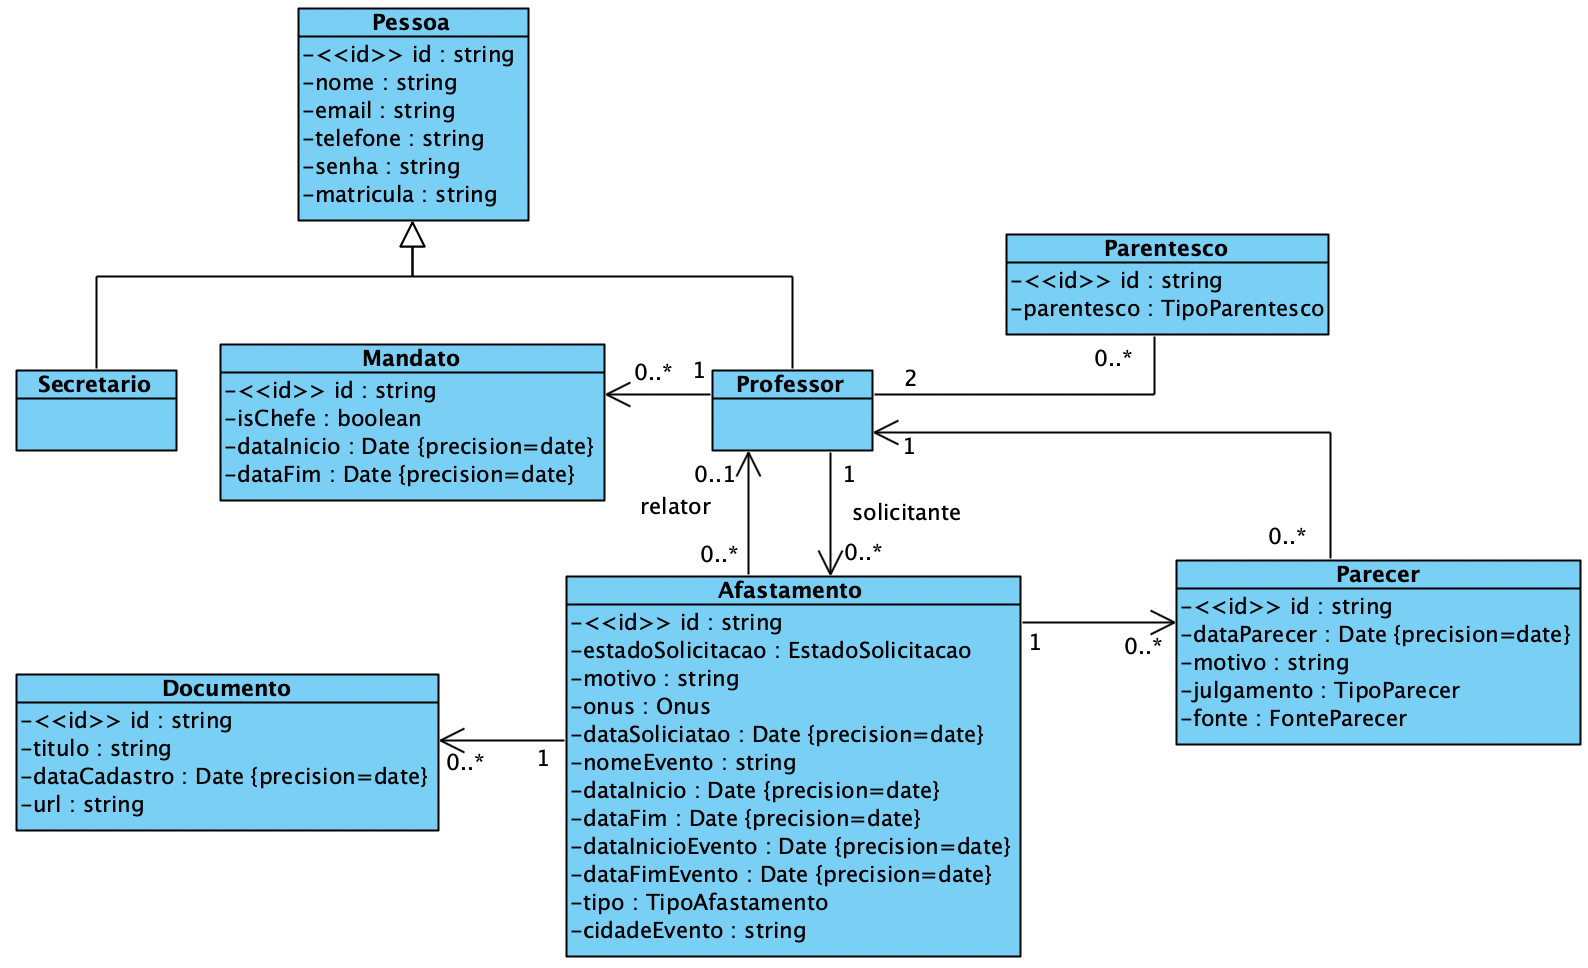
\includegraphics[width=1\textwidth]{figuras/fig-modelo-entidades.png}
    \caption{Modelo de Entidades do SCAP.}
    \label{fig-modelo-entidades}
\end{figure}

\vitor{Figura~\ref{fig-modelo-entidades}: 
	\begin{itemize}
		\item No TypeScript há um tipo de dado só pra datas e outro só pra horas ou existe apenas o \textsf{DateTime} usado no modelo? Se existir apenas um tipo unificado, é preciso especificar \textsf{precision=date} quando só estamos interessados na data (que é o caso na maioria das datas representadas no diagrama);
		\item As navegabilidades entre \textsf{Professor} e \textsf{Parentesco} foram pensadas pra ser desta forma mesmo? O objeto \textsf{p1} da classe \textsf{Professor} teria um atributo \textsf{parentesco} que se refere a uma instância da classe \textsf{Parentesco} que, por sua vez, tem um atributo \textsf{professor} que aponta para um objeto \textsf{p2} da classe \textsf{Professor}, mas \textsf{p2} não tem uma referência para este parentesco... Não seria melhor modelar como uma relação única \textsf{Professor} 2 -- 0.* \textsf{Parentesco}? A navegabilidade neste caso poderia ser dupla ou de \textsf{Parentesco} pra \textsf{Professor} apenas, pois essa informação é usada apenas num momento muito específico.
	\end{itemize}}

\sophie{Fiz as duas alterações}

\begin{figure}
    \centering
    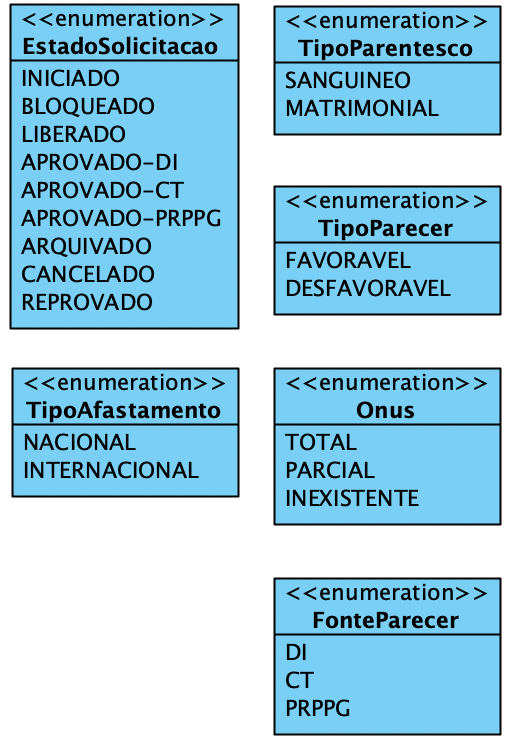
\includegraphics[width=0.5\textwidth]{figuras/fig-modelo-entidades-enum.png}
    \caption{Tipos Enumerados do Modelo de Entidades do SCAP.}
    \label{fig-modelo-entidades-enum}
\end{figure}


\subsection{Modelo de Persistência}
\label{subsec-frameweb-persistencia}

O modelo de persistência de FrameWeb é um diagrama de classes UML que representa
as classes responsáveis pela persistência das classes de domínio no banco de dados~\cite{souza:2007}.
Foi utilizado o padrão \textit{Repository} para a implementação das classes de persistência,
este propõe uma camada de separação entre o domínio e o mapeamento de dados.

\sophie{Acho que o get com filtros pode ser do IBaseRepositoy mas não ser definido em BaseRepository (filtros vão ser específicos de cada entidade)}


Para isso, foi criada uma interface base (\textbf{IBaseRepositoy}) que define os métodos comuns a todas as classes de persistência,
sendo eles: \textit{get} para buscar todos os elementos com base nos filtros passados como parâmetro,
\textit{post} para criar um novo elemento, \textit{getById} para buscar um elemento a partir de seu
\textit{id} e \textit{delete}. A Figura~\ref{fig-modelo-persist-base} apresenta essa interface e a
classe \textit{Repository} que a implementa. O tipo genérico \textit{T} representa a classe de domínio
sendo manipulada, ou seja, em \textbf{AfastamentoRepository} o método \textit{getById}
retorna um elemento da classe \textbf{Afastamento}.


\begin{figure}[h!]
    \centering
    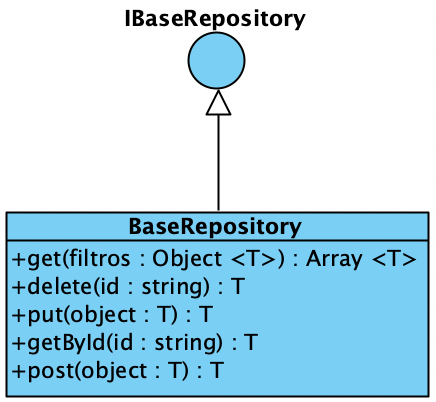
\includegraphics[width=0.4\textwidth]{figuras/fig-modelo-persist-base.png}
    \caption{Interface e Implementação do Repository Base.}
    \label{fig-modelo-persist-base}
\end{figure}


As interfaces do modelo herdam \textbf{IBaseRepositoy}, enquanto as classes \textit{Repository} estendem a
classe \textbf{BaseRepository}. De modo que todas as classes de persistência possuam, além dos métodos
específicos dessas, os métodos comuns definidos na interface base. As Figuras~\ref{fig-modelo-persist}
apresentam o modelo de persistência do SCAP.

\begin{figure}[h!]
    \centering
    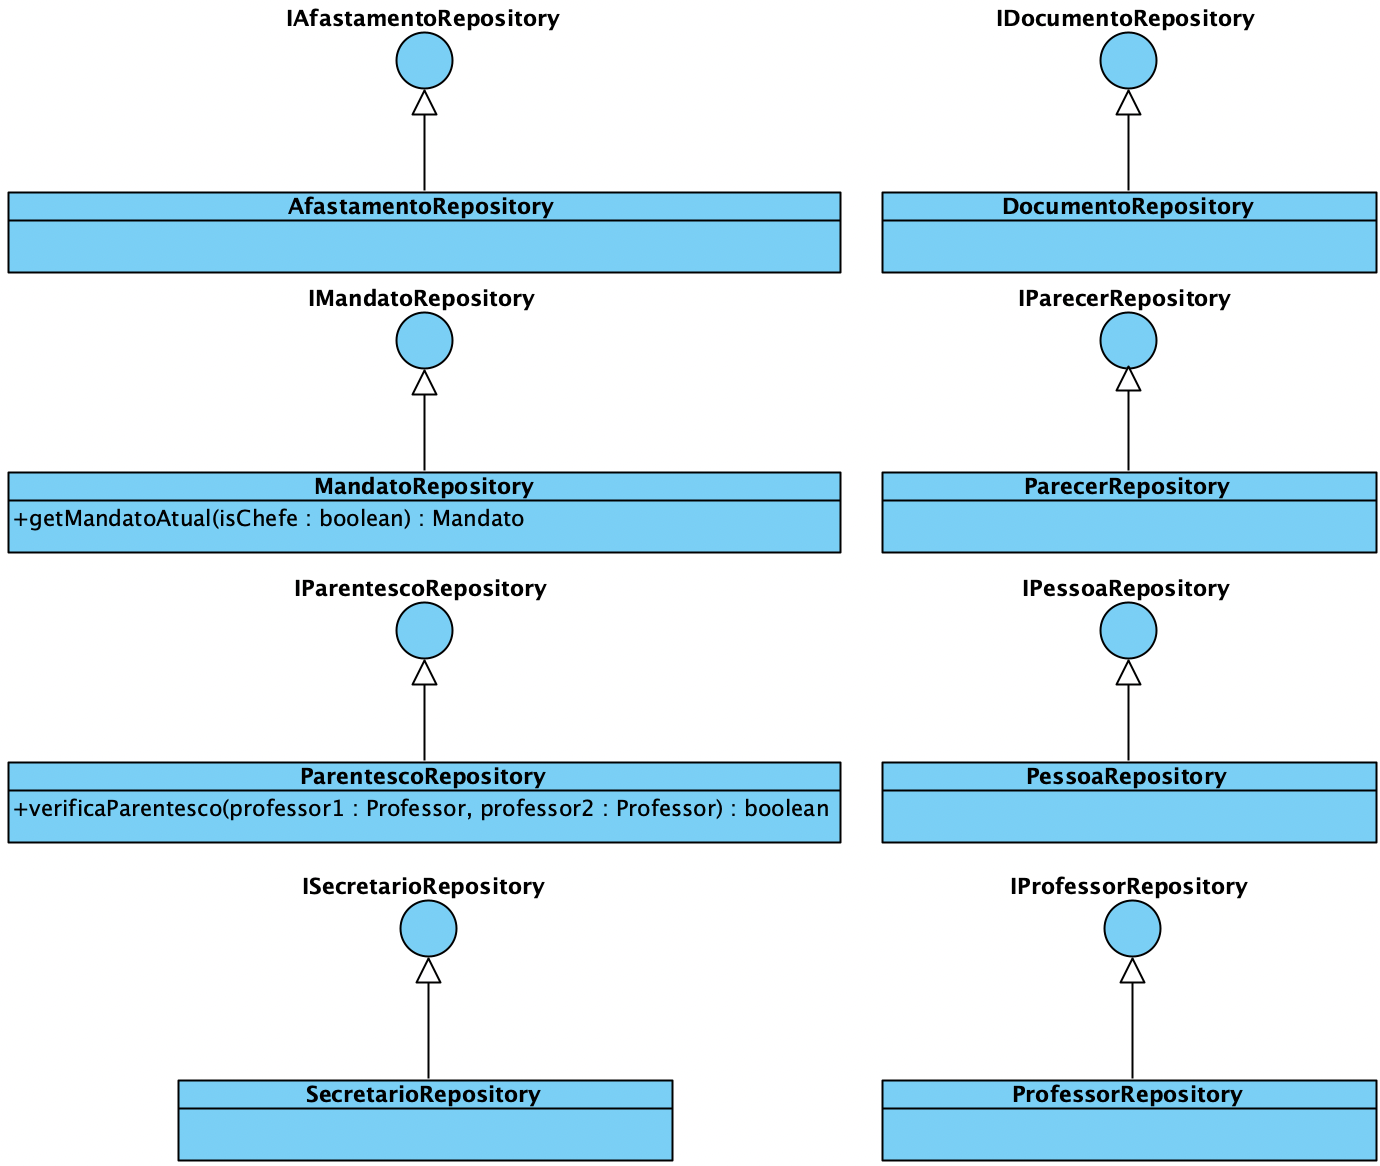
\includegraphics[width=0.9\textwidth]{figuras/fig-modelo-persist.png}
    \caption{Modelo de Persistência do SCAP.}
    \label{fig-modelo-persist}
\end{figure}

\vitor{Figura~\ref{fig-modelo-persist}: são só esses métodos mesmo que você precisou na implementação? Caso ainda vá avançar na implementação e surja a necessidade de novos métodos nos repositories, adicione-os neste modelo. 
	
	Além disso, o padrão de nome das interfaces é curioso. Eu imaginaria que a interface de \textsf{PessoaRepository} fosse \textsf{IPessoaRepository} e não apenas \textsf{IPessoa}. Esse é o padrão sugerido pelo \textit{framework} mesmo?}

\sophie{Por enquanto só esses métodos, mas se precisar de mais métodos adiciono aqui sim.
    Sobre o padrão de nomes, pesquisando sobre o Repository Pattern vi que não existe um consenso em relação ao nome das interfaces e classes, mas achei que de fato ficou mais claro nomear as interfaces com o sufixo Repository.}

\subsection{Modelo de Navegação}
\label{subsec-frameweb-navegacao}

O Modelo de Navegação é um diagrama de classe da UML que representa os diferentes componentes que
formam a camada de Lógica de Apresentação, como páginas Web, formulários HTML e classes de ação do \textit{framework} específico~\cite{souza:2007}. 
Esse modelo é utilizado para guiar a implementação dos pacotes Visão e Controle.

A Tabela~\ref{tab-estereotipos-navegacao} apresenta os estereótipos UML utilizados no modelo de navegação do SCAP,
propostos por~\citeonline{hoppe:2023} como uma adaptação, para \textit{frameworks} SPA,
dos estereótipos propostos originalmente por~\citeonline{souza:2007}.

\begin{table}[h!]
    \centering
    \caption{Estereótipos UML para Modelos de Navegação~\cite{hoppe:2023}.}
    \label{tab-estereotipos-navegacao}
    \begin{tabular}{|p{3cm}|p{12cm}|}
        \hline
        \textbf{Estereótipo} & \textbf{Descrição} \\
        \hline
        (Nenhum)    & Controladora de um framework Front Controller ou a parte controladora de um component de um framework SPA. \\
        \hline
        <<Page>>    & Página Web estática ou dinâmica. \\
        \hline
        <<Partial>> & Parte de uma página HTML que é gerada em tempo de execução por meio de AJAX. \\
        \hline
        <<Form>>    & Formulário HTML \\
        \hline
    \end{tabular}
\end{table}

A Figura~\ref{fig-modelo-navegacao-afast} apresenta o modelo de navegação do SCAP para os casos de uso
\textbf{Cancelar Afastamento}, \textbf{Cadastrar Afastamento} e \textbf{Consultar Afastamento}.

\begin{figure}
    \centering
    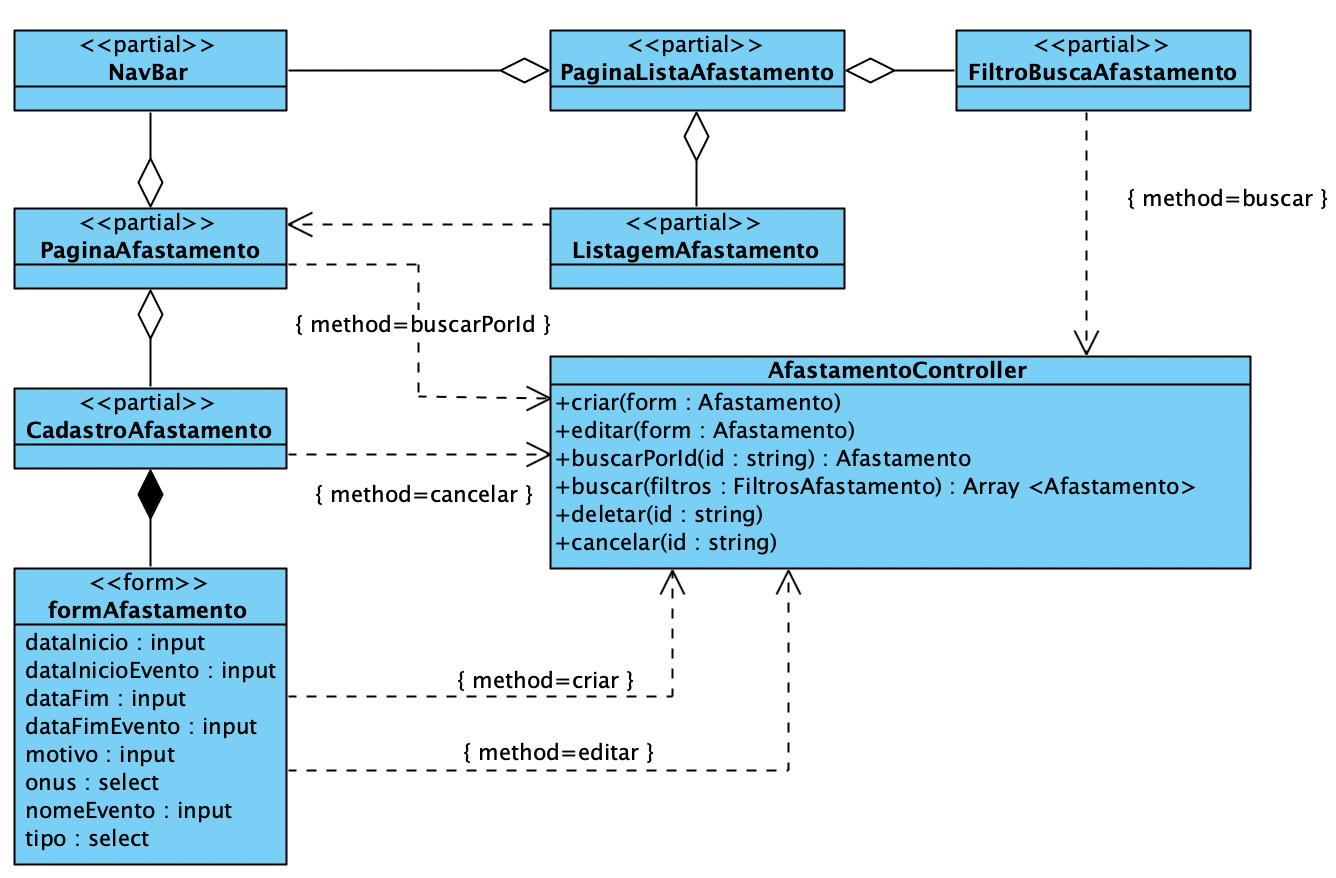
\includegraphics[width=1\textwidth]{figuras/fig-modelo-naveg-afast.png}
    \caption{Modelo de Navegação do SCAP.}
    \label{fig-modelo-navegacao-afast}
\end{figure}

A \textbf{PaginaListaAfastamento} é responsável por listar os afastamentos cadastrados.
Ela possui um componente filtro (\textbf{FiltroBuscaAfastamento}), em que é possível buscar
os afastamentos por diferentes critérios, definidos pela interface mostrada na Figura~\ref{fig-interface-filtro-afast}.
O componente \textbf{ListagemAfastamento} consiste de uma tabela que lista os afastamentos buscados,
cada linha da tabela possui um botão que redireciona para a página de detalhes do afastamento (\textbf{PaginaAfastamento}).

\begin{figure}
    \centering
    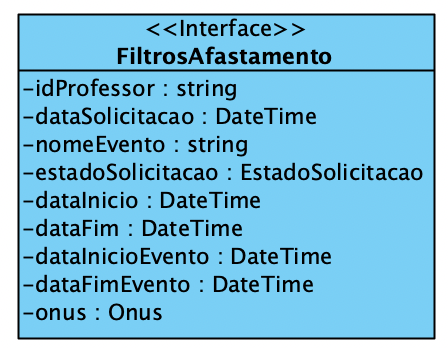
\includegraphics[width=0.4\textwidth]{figuras/fig-interface-filtro-afast.png}
    \caption{Interface Filtro Afastamento.}
    \label{fig-interface-filtro-afast}
\end{figure}

Se redirecionado para a \textbf{PaginaAfastamento} a partir do componente \textbf{ListagemAfastamento},
o \textit{partial} possui o atributo \textbf{id} inicializado com o \textit{id} do afastamento, e é
utilizado para fazer uma chamada ao método \textbf{buscarPorId} da \textit{controller} \textbf{AfastamentoController}.
Caso o usuário seja o solicitante do afastamento, ele pode cancelá-lo clicando em um botão que faz uma chamada ao método
\textbf{cancelar} da \textit{controller} \textbf{AfastamentoController}.

Quando não possui um \textit{id} inicializado, o \textit{partial} é utilizado para criar um novo afastamento,
o usuário deve então preencher os campos do formulário e clicar em um botão que faz uma chamada ao método
\textbf{criar} da \textit{controller} \textbf{AfastamentoController}.


\begin{figure}
    \centering
    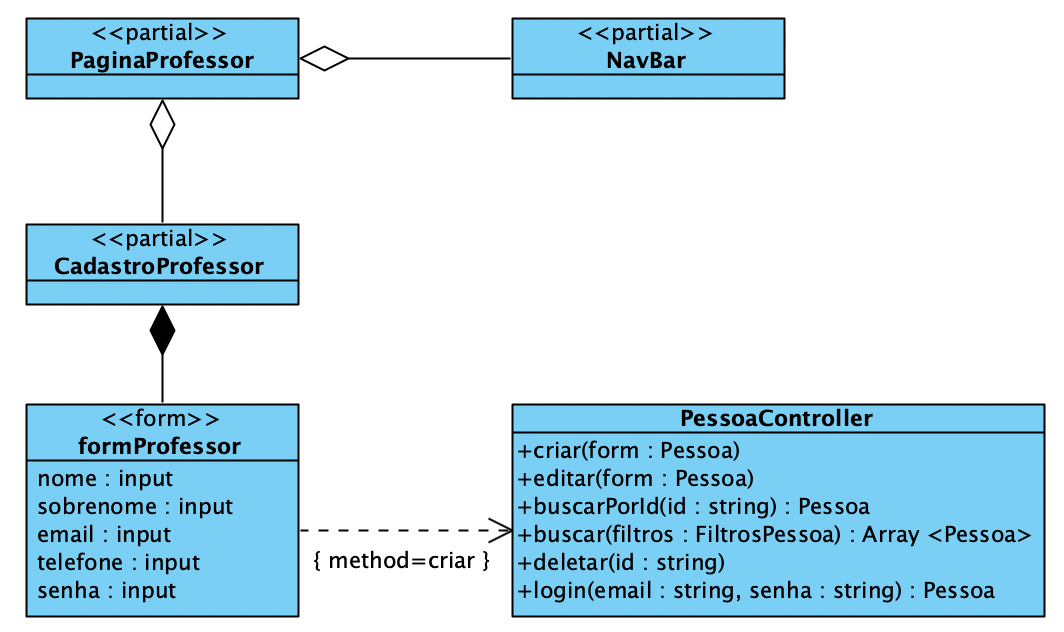
\includegraphics[width=0.9\textwidth]{figuras/fig-modelo-naveg-cadast.png}
    \caption{Modelo de Navegação do SCAP do Caso de Uso Cadastrar Professor.}
    \label{fig-modelo-navegacao-professor}
\end{figure}

A Figura~\ref{fig-modelo-navegacao-professor} apresenta o modelo de navegação do SCAP para o caso de uso
\textbf{Cadastrar Professor}. Na \textbf{PaginaProfessor} o secretário pode cadastrar um novo professor,
para isso ele deve preencher os campos do formulário e clicar em um botão que faz uma chamada ao método
\textbf{criar} da \textit{controller} \textbf{PessoaController}.

\vitor{Explicar o componente \textsf{NavBar} presente nas duas figuras.}

O componente \textbf{NavBar} presente em ambos os modelos de navegação é responsável por exibir
no topo da tela uma barra de navegação com links para as páginas principais do sistema, como a página inicial,
a página de listagem de afastamentos e a página de cadastro de professores. Ele é um componente
comum a todas as páginas do sistema, exceto à tela de \textit{login}.

\subsection{Modelo de Aplicação}
\label{subsec-frameweb-aplicacao}
O Modelo de Aplicação é um diagrama de classes da UML que representa as classes de
serviço, que são responsáveis pela codificação dos casos de uso, e suas dependências~\cite{souza:2007}.
Por ele pode-se visualizar a dependência entre os pacotes Controle (classes de ação),
Aplicação (classes de serviço) e Persistência (interfaces \textit{Repository}). 

As figuras~\ref{fig-modelo-aplicacao-1} e~\ref{fig-modelo-aplicacao-2} contém os Modelos de Aplicação.
As solicitações dos usuários são tratadas pelas classes de controle, que por sua vez
chamam as classes de serviço para realizar as operações de negócio, que por fim acessam
as classes de persistência para realizar as operações de leitura e escrita no banco de dados.


\begin{figure}[h!]
    \centering
    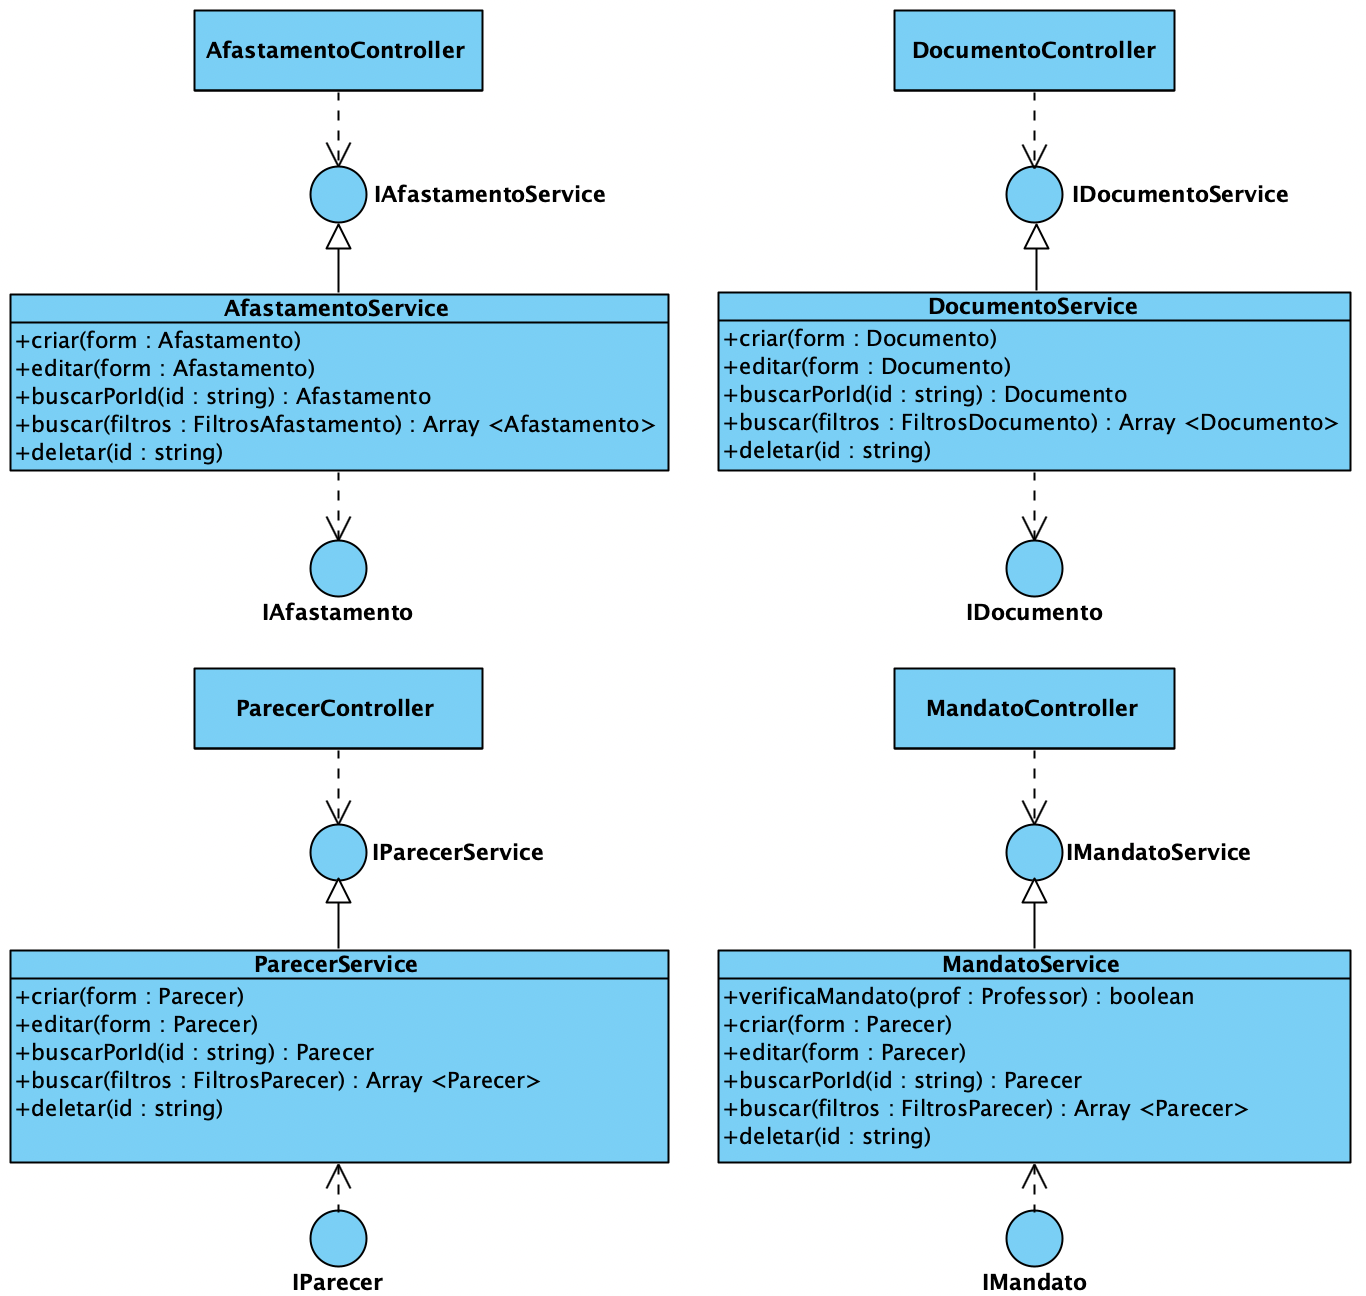
\includegraphics[width=0.9\textwidth]{figuras/fig-modelo-apl-1.png}
    \caption{Modelo de Aplicação do SCAP.}
    \label{fig-modelo-aplicacao-1}
\end{figure}

\vitor{Figura~\ref{fig-modelo-aplicacao-1}: acredito ue a direção da dependência entre \textsf{IParecer} e \textsf{ParecerService} esteja invertida, idem para \textsf{IMandato}. Além disso, foi usada uma relação de dependência entre as classes (controlador-serviço e serviço-repository). O FrameWeb geralmente usa uma associação entre essas classes, mas pode ser porque no Java, que é meu background, as classes de fato possuem um atributo que é uma referência pra outra classe. No seu caso uma dependência representa isso melhor? Se sim, inclua no texto uma explicação sobre isso.}
\sophie{Consertei as direções e verifiquei que a associação é mais adequada mesmo, então mudei para associação.}

\begin{figure}[h!]
    \centering
    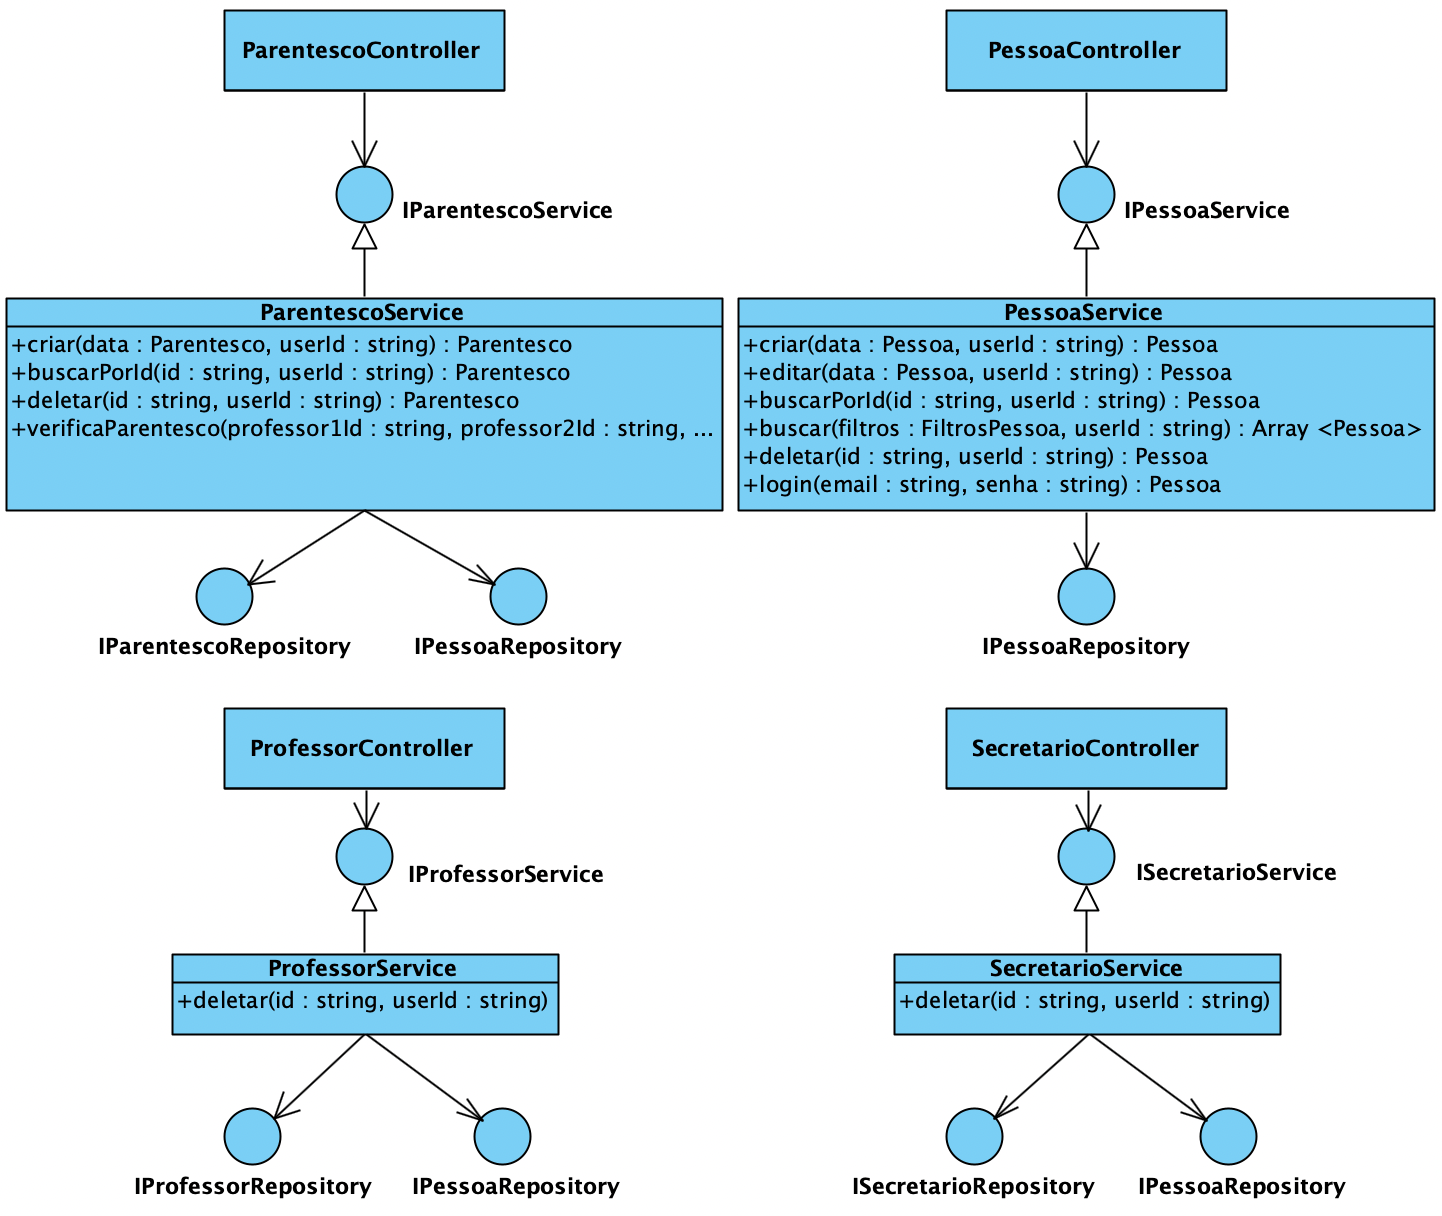
\includegraphics[width=0.9\textwidth]{figuras/fig-modelo-apl-2.png}
    \caption{Modelo de Aplicação do SCAP.}
    \label{fig-modelo-aplicacao-2}
\end{figure}


\section{Implementação e Resultados}
\label{sec-projeto-impl}

Essa seção apresenta a implementação do SCAP, por meio de capturas de tela,
e discute os resultados obtidos.